\documentclass[PianoDiQualifica.tex]{subfiles}

\begin{document}
%http://www.praxiom.com/iso-90003.htm citato da Tullio può servire come base per capire processi meglio
\chapter{Qualità di processo}

\section{Scopo} 
Per garantire la qualità del prodotto è necessario perseguire la qualità dei processi che lo definiscono.
Per raggiungere questo obiettivo, si è deciso di seguire il principio di miglioramento continuo (PDCA) e di adottare lo standard ISO/IEC 15504 denominato SPICE (Software Process Improvement and Capability Determination).

\section{Procedure di controllo di qualità di processo}
La qualità dei processi verrà garantita dall'applicazione del principio PDCA, descritto dell'appendice A. Grazie a questo principio, sarà possibile ottenere un miglioramento continuo della qualità di tutti i processi, inclusa la verifica, e come diretta conseguenza si otterrà il miglioramento dei prodotti risultanti. 

Per ottenere qualità dei processi, bisogna:
\begin{itemize}
	\item Definire il processo: affinché sia controllabile;
	\item Controllare il processo: in funzione dell'ottenimento di efficacia, efficienza ed esperienza;
	\item Usare buoni strumenti di valutazione: SPICE e PDCA;
\end{itemize}

\section{Metriche per i processi}%VERI-GIORAT non più metriche ma solo processi siccome di seguito elencata lista dei processi e all'interno di ogni processo le sue metriche.

%VERI-GIORAT corrette le metriche e le appendici.
%manca la citazione di un qualsiasi processo che abbiamo gestito, guardando dai processi analizzati da altri gruppi direi che noi durante la RR dovremmo avere almeno questi:

%VERI-GIORAT non so se sia citato veramente da ISO/IEC 15504 o da  IEEE STD 12207-2008 siccome non trovo indici disponibili 
\subsection{Processo di pianificazione di progetto, impostazione e controllo processi}
Il macro-processo ha lo scopo di produrre dei piani di sviluppo per il progetto, comprendenti
la scelta del modello di ciclo di vita del prodotto, descrizioni delle attività e dei compiti
da svolgere, pianificazione temporale del lavoro e dei costi da sostenere, allocazione di compiti e
responsabilità, e misurazioni per rilevare lo stato del progetto rispetto alle pianificazioni prodotte.
%VERI-GIORAT le metriche da te descritte fanno parte di solo questo processo che è come un master per tutti i processi che sono branch diciamo 
\subsubsection{Obiettivi}
Sviluppo del progetto dovrà.... ponendo in enfasi:
\begin{itemize}
	\item \textbf{Rispetto budget:} blah blah 
	\item %VERI-GIORAT lavoro del singolo e segnalazione preventiva problemi di ritardo consegna task membri
\end{itemize}

\subsubsection{Strategie}
Ogni eventuale valore negativo a livello di Schedule o Budget Variance rilevato sarà compensato....

\subsubsection{Metirche} %VERI-GIORAT ho messo le due metriche che avevi scritto dentro al processo di appartenenza
\paragraph{Schedule Variance (SV)}
Indica se si è in linea, in anticipo o in ritardo rispetto alla schedulazione delle attività di progetto pianificate nella baseline.\\
È un indicatore di efficacia soprattutto nei confronti del Cliente. \\
Se SV è positivo, significa che il progetto sta producendo con maggior velocità rispetto a quanto pianificato, viceversa se negativo.
%VERI-GIORAT: ogni metrica deve avere una misurazione matematica/formula
%inoltre deve essere presente un range ottimale e di accettazione messo nella tabella riassuntiva alla fine della qualità di processo come come è stato fatto per la qualità di prodotto.
\textbf{Misurazione:}


\paragraph{Budget Variance (BV)}
Indica se alla data corrente si è speso di più o di meno rispetto a quanto previsto a budget alla data corrente.\\
È un indicatore che ha un valore unicamente contabile e finanziario.\\
Se BV è positivo significa che il progetto sta spendendo il proprio budget con minor velocità di quanto pianificato, viceversa se negativo.
%VERI-GIORAT: ogni metrica deve avere una misurazione matematica/formula
%inoltre deve essere presente un range ottimale e di accettazione messo nella tabella riassuntiva alla fine della qualità di processo come come è stato fatto per la qualità di prodotto.
\textbf{Misurazione:}



%VERI-GIORAT stesso discorso che per il processo precedente spiegando che questo è pianficiato come processo futuro da attivare durante progettazione
\subsection{Processo verifica software}
Il processo punta a verificare se qualsiasi elemento del sistema soddisfa completamente i requisiti ad esso correlati.
%VERI-GIORAT processo per garantire ogni parte documentazione chiara e migliorabile/misurabile
\subsubsection{Obiettivi}
....
 \begin{itemize}
 	\item \textbf{Obiettivo 1 bla:} blah blah 
 \end{itemize}
 
\subsubsection{Strategie}
%VERI-GIORAT Utilizzo di tool come Sonarlint Sonarcloud ecc guardando dalle norme
 
\subsubsection{Metirche}
\paragraph{Branch Coverage}%VERI-GIORAT Branch Coverage e Code Coverage essendo stati citati nelle ultime lezione da Tullio
\paragraph{Code Coverage}

%VERI-GIORAT: ogni metrica deve avere una misurazione matematica/formula
%inoltre deve essere presente un range ottimale e di accettazione messo nella tabella riassuntiva alla fine della qualità di processo come come è stato fatto per la qualità di prodotto.
\textbf{Misurazione:}



\section{Tabella delle metriche}
% ID METRICA
% M --> metrica
% PS--> processo
% (lettera per macro categoria, se esistono)
% 00n --> numero incrementale
Questa tabella indica i \textbf{range} di accettazione e di ottimalità per le metriche utilizzate per la qualità di processo:
\begin{table}[H]
	\begin{center}
		\begin{tabu} to \textwidth {
			>{\centering}m{0.15\linewidth}
			>{\centering}m{0.45\linewidth}
			>{\centering}m{0.18\linewidth} 
			>{\centering\arraybackslash}m{0.17\linewidth}
			}
			\tableHeaderStyle
			\textbf{ID} & \textbf{Nome} & \textbf{Range di accettazione} & \textbf{Range di ottimalità}\\

			MPS...001 & ... & ... & ... \\ 

		\end{tabu}
		\caption{Tabella delle metriche della qualità di processo}
		\vspace{-1em}
	\end{center}
\end{table}




\begin{appendices}

\chapter{Ciclo di Deming o PDCA}
Ogni processo deve essere organizzato basandosi sul principio del miglioramento continuo (o ruota di Deming):
\begin{description}
	\item [Plan] (pianificare): viene definito un piano che parte dalla definizione di problemi e obiettivi, pianifica compiti, assegna responsabilità, studia il caso, analizza le cause della criticità, definisce azioni correttive; 
	\item [Do](eseguire): vengono implementate le attività secondo le linee definite durante la fase Plan;
	\item [Check] (valutare): viene verificato l'esito delle azioni di miglioramento rispetto alle attese;
	\item [Act] (agire): vengono applicate le correzioni necessarie per colmare le carenze rilevate, e vengono standardizzate le attività correttamente eseguite.
\end{description}

\begin{figure}[htbp]
	\begin{center}
		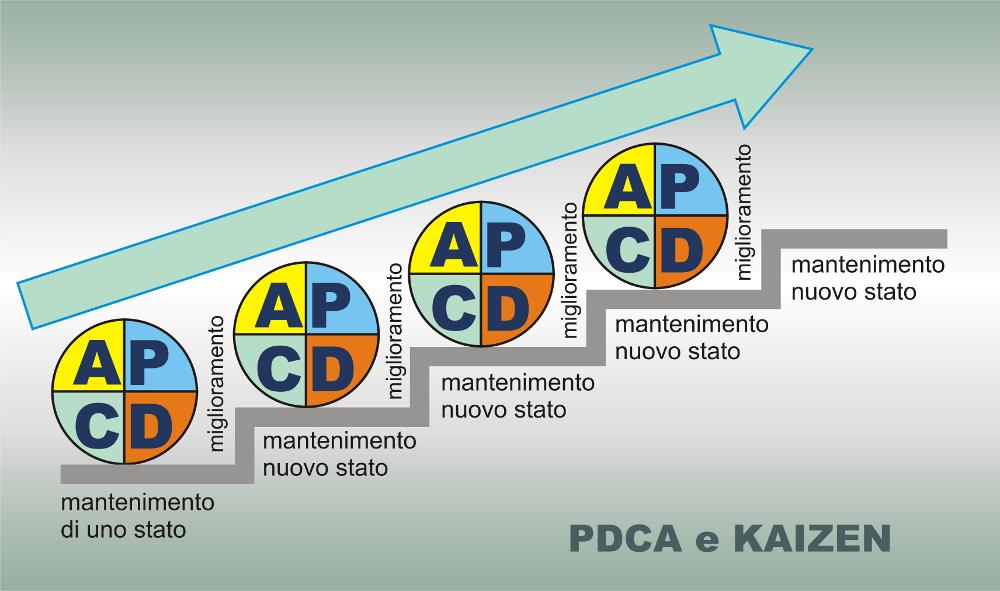
\includegraphics[width=0.7\linewidth]{../../common/images/PDCAkaizen}
		\caption[Ciclo di Deming]{Ciclo di Deming}
		\label{fig:pdca}
	\end{center}
\end{figure}

\chapter{ISO/IEC 15504}
Lo standard ISO/IEC 15504 contiene un modello di riferimento che definisce 
\begin{itemize}
	\item Process dimension;
	\item Capability dimension.
\end{itemize}

La dimensione di processo divide i processi in cinque categorie:
\begin{itemize}
	\item Customer-supplier;
	\item Engineering;
	\item Supporting;
	\item Management;
	\item Organization.
\end{itemize}

Per ogni processo, lo standard ISO/IEC 15504 definisce dei livelli di capacità:
\begin{description}
	\item [\normalfont Livello 5] \textbf{Optimizing process}: il processo è continuamente migliorato;
	\item [\normalfont Livello 4] \textbf{Predictable process}: il processo è adottato sistematicamente, entro limiti definiti;
	\item [\normalfont Livello 3] \textbf{Established process}: un processo stabilito si basa su un processo standard;
	\item [\normalfont Livello 2] \textbf{Managed process}: il processo è gestito e i prodotti sono stabiliti, controllati e mantenuti;
	\item [\normalfont Livello 1] \textbf{Performed process}: il processo è implementato e raggiunge lo scopo stabilito;
	\item [\normalfont Livello 0] \textbf{Incomplete process}: il processo non è implementato o non raggiunge lo scopo stabilito.\\
\end{description}

La capacità dei processi viene misurata attraverso degli attributi di processo.
\begin{description}
%VERI-GIORAT mettere per ogni processo un numero che indichi il livello di processo a cui appartiene per rendere facile l'individuamento del livello del processo tramite i seguenti attributi? Idea
\item [Process performance:] capacità di un processo di raggiungere gli obiettivi trasformando input identificabili in output identificabili;
\item [Performance management:] capacità del processo di elaborare un prodotto coerente con gli obiettivi fissati;
\item [Work product management:] capacità del processo di elaborare un prodotto documentato, controllato e verificato;
\item [Process definition:] l'esecuzione del processo si basa su standard di processo per raggiungere i propri obiettivi;
\item [Process deployment:] capacità del processo di attingere a risorse tecniche e umane appropriate per essere attuato efficacemente;
\item [Process measurement:] gli obiettivi e le misure di prodotto e di processo vengono usati per garantire il raggiungimento dei traguardi definiti in supporto ai target aziendali;
\item [Process control:] il processo viene controllato tramite misure di prodotto e processo per effettuare correzioni migliorative al processo stesso;
\item [Process innovation:] i cambiamenti strutturali, di gestione e di esecuzione vengono gestiti in modo controllato per raggiungere i risultati fissati;
\item [Process optimization:] le modifiche al processo sono identificate e implementate per garantire il miglioramento continuo nella realizzazione degli obiettivi di business dell'organizzazione. 
\end{description}

Ogni attributo consiste di una o più pratiche generiche che sono ulteriormente elaborate in indicatori pratici per aiutare la valutazione delle performance, sotto forma di indici N-P-L-F:
\begin{itemize}
	\item Non soddisfatto (0 - 15\%);
	\item Parzialmente soddisfatto ($ > $15\% - 50\%);
	\item Largamente soddisfatto ($ > $50\% - 85\%);
	\item Totalmente soddisfatto ($ > $85\% - 100\%)
\end{itemize}

\end{appendices}
\end{document}